\section{Unit tests}
At teste ved at lave udskrifter i consolen er dumt, så nu laver vi unit tests. En unittest er en test af et enkelt modul i koden. Vi tester vores kode for at fange fejl på et tidligt stadie. Når man skriver tests, tvinges man samtidig til at tænke mere over koden man har skrevet.

\begin{itemize}
	\item \textbf{Unit test} - Et stykke kode, typisk en metode, der bruger et andet stykke kode for at teste nogen antagelsers korrekthed.
	\item \textbf{Unit} - En metode.
	\item \textbf{System Under Test} - Det system man tester på.
\end{itemize}

\paragraph{En god Unittest}
\begin{itemize}
	\item Automatiseret og gentagelig.
	\item Skal køre hurtigt.
	\item Skal kunne køres blot ved hjælp af et tryk på en knap.
	\item Skal køre isoleret fra andre tests.
	\item Ved fejl skal det tydeligt fremgå hvad der er gået galt.
\end{itemize}

\subsection{Blackbox vs. Whitebox}
To grundlæggende forskellige måder at teste på:

\begin{table}[H]
	\begin{tabular}{ll}
		\textbf{Whitebox} & Bedst egnet til unittest for udviklere med kendskab til implementering.\\
		\textbf{Blackbox} & Egnet til QA\footnote{Quality Assurance.} testere, uden kendskab til specifik implementering.\\
	\end{tabular}
\end{table}

Det er vigtigt at vi tester systemet, ''set udefra'', så vores test ikke bliver afhængige af implementeringen. Eksempelvis er det en dårlig ide at gøre variabler og lignende \textit{public} for at kunne teste dem.

\subsection{Hvordan unittester vi?}
Vi bruger testframeworket NUnit, hvilket giver mulighed for:

\begin{itemize}
	\item Detaljerede fejlrapporter - beskriver hvorfor en test fejler.
	\item Setup og teardown, se Code listing~\ref{code:nunit}.
	\item At nemt indsætte nye tests i systemet.
\end{itemize}

\subsubsection{NUnit attributter}
NUnit bruger en række 'tags' som indikerer hvordan den skal udføre de skreve test. Nogle af disse er vist i tabel~\ref{tab:nunit}.

\begin{table}[H]
	\centering
	\begin{tabular}{ll}
		\toprule
		\textbf{Attribut}& 	\textbf{Beskrivelse}\\ \midrule
		TestFixture	&	En klasse der indeholder automatiserede NUnit tests. \\
		SetUp		&	Køres hver gang en test i samme TestFixture køres.\\
		TearDown	&	Køres hver gang en test i samme TestFixture er afsluttet.\\
		Test		&	En enkelt automatiseret test.\\
		TestCase()	&	En test med parametre.\\ \bottomrule
	\end{tabular}
	\caption{NUnit's attributter (tags).}
	\label{tab:nunit}
\end{table}

Yderligere er der nogle konventioner man følger når testmetoder skal navngives, demonstreret på linje 15 i Code listing~\ref{code:nunit}.

\paragraph{Opsætning af unittest} Når der skrives en Unittest, følger man typisk de tre A'er.

\begin{enumerate}
	\item Arrange - Instantiering af UUT objekt.
	\item Act - Stimuler UUT til at gøre det vi ønsker - \textit{result = \_uut.Method()}.
	\item Assert - Assertion på om vi får det forventede resultat. \textit{Assert.False(result)}.
\end{enumerate}

\begin{lstlisting}[caption=NUnit eksempel på Setup og Teardown.,label=code:nunit]
[TestFixture]
public class MyClassUnittest {

	[SetUp]
	public void Setup() {
		// happens before each test
	}
	
	[TearDown]
	public void Teardown() {
		// happens after each test
	}
	
	[Test]
	public void MethodName_WhatTotestFor_ExpectedResult() {
		// assert something here
	}
}
\end{lstlisting}

%\subsubsection{Parametiserede tests}
%I NUnit er der mulighed for at at bruge parametiserede tests. Dette er nyttigt hvis man ønsker at køre samme test med flere forskellige parametre. I stedet for at bruge \textbf{Test} attributten, bruges \textbf{TestCase(arg1, arg2)} attributten.

%\begin{figure}[H]
%\centering
%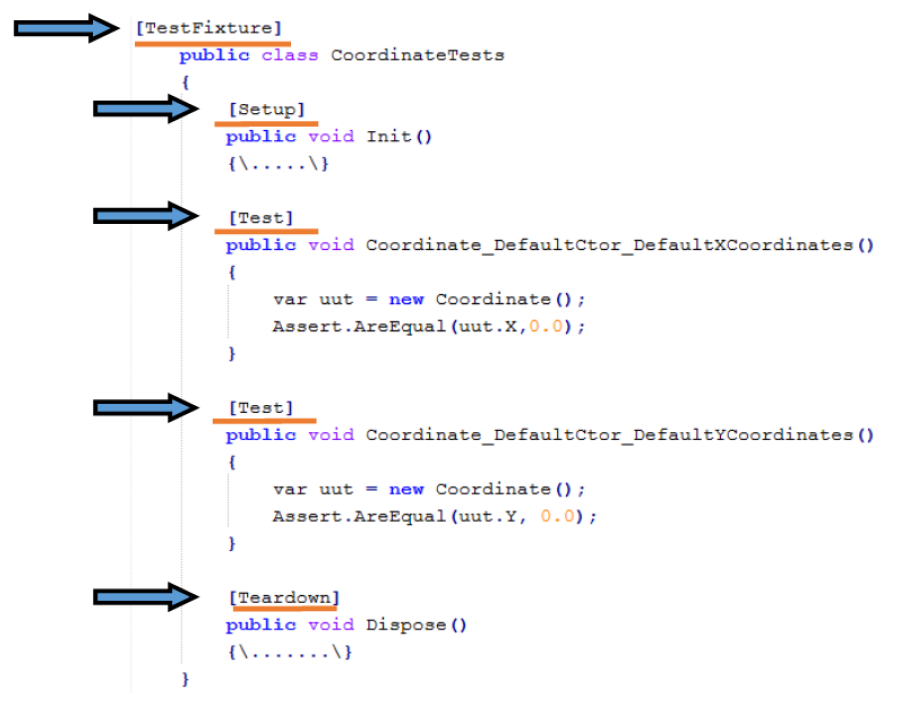
\includegraphics[width=0.7\linewidth]{figs/testFixture.PNG}
%\caption{Syntaks for unittesting i NUnit}
%\label{fig:testFixture}
%\end{figure}

\subsubsection{The Green Zone}
Adskil unittests fra andre komplicerede test, f.eks: integrationstest. Ved at lave denne seperation kan unittest i denne zone køres hurtigt og derved køres de oftere. Ved at have en \textit{safe \textcolor{green!80!black}{green} zone} får udviklere et sted hvor:

\begin{itemize}
	\item Only unittests are contained.
	\item They know that they can get the latest code version.
	\item They can run all tests in that namespace or folder, and they should all be green.
\end{itemize}

Hvis en test i \textit{the green zone} fejler, har man et problem.

\subsection{Assertion models}
Der findes to typiske måder at asserte på. Den ene kaldes den klassiske model og den anden kaldes Constraint baseret. I NUnit 3.0 er assertions primært skrevet med den contraint-baserede model, som tager et \textit{constaint object}, eksempelvis \textit{Is.EqualTo()} som argument.

\subsubsection{Classic assert model}

Den klassiske assert anvender \textit{AreEqual} metoden. Denne tager to argumenter, en værdi samt metoden som ønskes testet - her om den returnerer den korrekte værdi.

\begin{figure}[H]
\centering
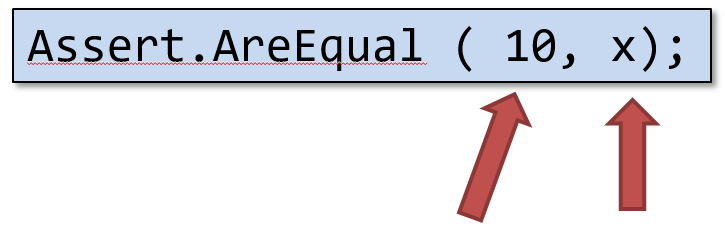
\includegraphics[width=0.4\linewidth]{figs/classicAssert.PNG}
\caption{Classic assert model.}
\label{fig:classicAssert}
\end{figure}

\subsubsection{Constraint-based assert model}
I en constraint-based model anvendes \textit{Assert.That()}. Denne bruger den faktiske værdi og et constraint, som \textit{Is.EqualTo("assumed result")}.

\begin{figure}[H]
\centering
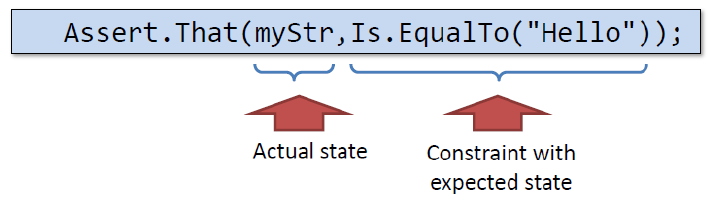
\includegraphics[width=0.5\linewidth]{figs/constraintAssert}
\caption{Constraint-based assert model.}
\label{fig:constraintassert}
\end{figure}





































